\documentclass[tikz,border=2pt]{standalone}
\usepackage{amsmath,amssymb}
\usepackage{pgfplots}
\pgfplotsset{compat=1.18}
\usetikzlibrary{calc}

\begin{document}
% The mode is where the density (or pmf) is highest: for f(x) = x e^{-x} it is x = 1, the
% most likely region, not the mean (2) nor the median (1.68).
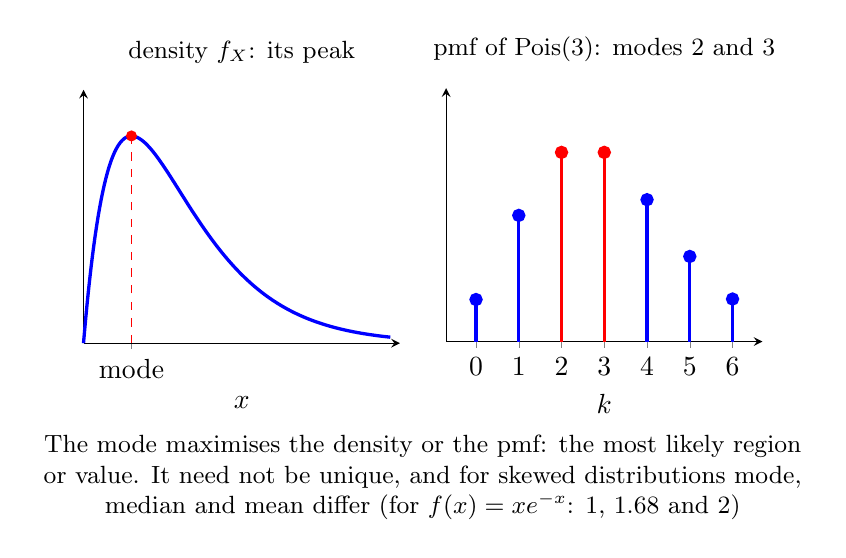
\begin{tikzpicture}
	\begin{axis}[
		name=p1, axis lines=left, xmin=0, xmax=6.6, ymin=0, ymax=0.45,
		xtick={1}, xticklabels={mode}, ytick=\empty,
		xlabel={$x$},
		samples=160, smooth, width=5.6cm, height=4.8cm, clip=false, title={density $f_X$: its peak}, title style={font=\small}
		]
		\addplot[blue, very thick, domain=0:6.4] {x*exp(-x)};
		\draw[red, dashed] (axis cs:1,0) -- (axis cs:1,0.368);
		\fill[red] (axis cs:1,0.368) circle (2pt);
	\end{axis}
	\begin{axis}[
		name=p2, at={(p1.outer east)}, anchor=outer west, xshift=3mm,
		axis lines=left, xmin=-0.7, xmax=6.7, ymin=0, ymax=0.3,
		xtick={0,...,6}, ytick=\empty,
		xlabel={$k$},
		width=5.6cm, height=4.8cm, clip=false, title={pmf of $\operatorname{Pois}(3)$: modes $2$ and $3$}, title style={font=\small}
		]
		\addplot[ycomb, blue, very thick, mark=*, mark size=1.8pt] coordinates {(0,0.0498) (1,0.1494) (4,0.1680) (5,0.1008) (6,0.0504)};
		\addplot[ycomb, red, very thick, mark=*, mark size=1.8pt] coordinates {(2,0.2240) (3,0.2240)};
	\end{axis}
	\node[anchor=north, font=\small, align=flush center, text width=9.8cm] at ([yshift=-2pt]$(p1.outer south)!0.5!(p2.outer south)$) {The mode maximises the density or the pmf: the most likely region or value. It need not be unique, and for skewed distributions mode, median and mean differ (for $f(x)=xe^{-x}$: $1$, $1.68$ and $2$)};
\end{tikzpicture}
\end{document}
